\chapter{Registration Pipeline using Line Features}
In this chapter we follow up on the definition of the Vector-valued Gaussian Model for 3D Face Registration by describing the registration pipeline built to put this concept into practice. The pipeline is of a sequential nature, where in each step the output of a data processing unit is the input for the next step. To enhance the registration outcome of this pipeline we use contour lines of key regions of the face. 
\section{Line Features}
\subsection{Definition of Line Features}
For every scan we want to register, 8 contours have been marked on three images of the face - taken from the front, the left and the right of the face - with a special GUI for marking points and lines on images. These contours depict the eyebrows, eyes, ears and lips of a face and we call them ``line features''. They are made up of a set of segments, each of  which is modelled with a \textbf{B\'{e}zier curve} (parametric curve frequently used in computer graphics, bernstein basis polynomials, used for
modelling smooth curves) of varying order. Due to the nature of the objects depicted, there are open as well as closed curves. 
\begin{equation}
    B(t)=\sum_{i=0}^{n}(1-t)^{n-i}t^iP_{i}
\end{equation}
The line features are saved in explicit files along with the face mesh of the scan.

\begin{comment}
\def\eyepath{(-3,0) .. controls (-2,1.8) and (2,2.2) .. (2.7,0) .. controls (2,-1.2) and (-2,-1.4) .. (-3,0)--cycle;}
\def\eyebrowpath{(3,0.5) .. controls (3,1.5) and (6.5,1.5) .. (7,0.5) .. controls (5.5,0) and (2,-0.5) .. (4.8,0.5);}

\begin{tikzpicture}
    \draw[black]\eyepath
    \draw[black]\eyebrowpath
\end{tikzpicture}

\viscomment{draw eye and eyebrow with bezier curves, first look at real world recorded images}
\end{comment}
\begin{figure}[h!]
    \centering
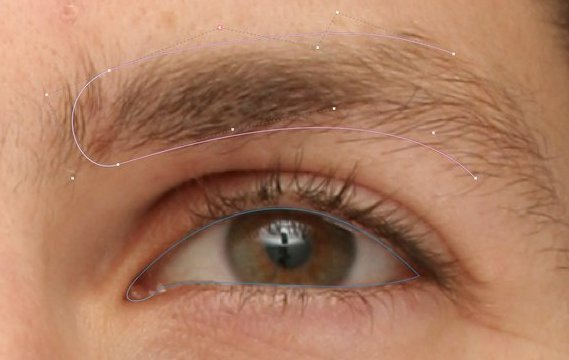
\includegraphics[width=\textwidth]{./resources/img/eyebrow_left.jpeg}
\caption{Line Features of the left eyebrow and eye, consisting of b\'{e}zier curves defined by visible control points (white)}
\end{figure}
\subsection{Why use Line Features for Registration?} 
Line features serve the purpose of augmenting the quality of registration by initiating it with a larger set of corresponding points (points which are on the lines). They are used to mark complex regions of the eyes, i.e. the eyes, ears etc., so that the registration process produces an accurate mapping of the contours of these organs which would otherwise not be possible.  Areas containing ``curves'' have a dense abundance of points/parameter changes, while straight areas only have scarce points.  

\section{Sampling 3D Points from 2D Line Features} 
In order to be able to use line features in the Vector-valued Gaussian Model, they have to be sampled at discrete intervals resulting in a set of additional landmarks $L_{Add} = \{l_{1}, \cdots, l_{N}\}$. These define the mapping $\Omega:L_{Add\mathcal{M}} \rightarrow L_{Add\mathcal{T}}$ of the contours - describing the different imporant features present in the faces - in the mean face mesh on those of the target face mesh. In order for the mapping $\Omega$ to be plausible, it is essential
for the curves to have equidistant parametrization so that when curves undergo sampling of N points, these N points are all at equal parametric intervals.

\def\earpathf{(-1,1.5) .. controls (-1,2.3) and (1,2.8) .. (1,1.5) .. controls (1, -.2) and (0.3,-.1) .. (0.3,-1) .. controls (0.2,-1.5) and (-.5, -1.7) .. (-1,-1.25);}
\def\earpathl{(3,2) .. controls (3,3.3) and (5.6,3.7) .. (5.6,2) .. controls (5.6, 0) and (4.6,0) .. (4.6,-1.3) .. controls (4.6,-2) and (3.5, -2) .. (3,-1.5);}
\begin{figure}[h!]
    \centering
    \begin{tikzpicture}
        \draw[black]\earpathf
        \fill (-1,1.5) circle[radius=2pt];
        \fill (0.1,2.3) circle[radius=2pt];
        \fill (1,1.5) circle[radius=2pt];
        \fill (0.8, 0.25) circle[radius=2pt]; 
        \fill (0.3,-1) circle[radius=2pt];
        \fill (-1,-1.25) circle[radius=2pt];
        \draw[black]\earpathl
        \fill (3,2) circle[radius=2pt];
        \fill (4.3, 3.12) circle[radius=2pt];
        \fill (5.6,2) circle[radius=2pt];
        \fill (5.25,0.35) circle[radius=2pt];
        \fill (4.6,-1.3) circle[radius=2pt];
        \fill (3,-1.5) circle[radius=2pt];
        \draw[ultra thick, blue, ->] (-.8,1.5) -- (2.8,2);
        \draw[ultra thick, blue, ->] (1, 0.25) -- (5.1, 0.35);
        \draw (1.8, .9) node {\Large\textcolor{blue}{$\Omega$}};
        \draw (-1,.5) node {line feature of $\mathcal{M}$};
        \draw (4,1.2) node {line feature of $\mathcal{T}$};
    \end{tikzpicture}
    \label{fig:DiffEars}
    \caption{Mapping of equidistant samples of \textbf{ear} line features from the reference (left) on to the target (right)}
\end{figure}

\subsection{Arc Length Parametrization}
The first problem which becomes apparent when trying to sample the line features is that the b\'{e}zier curve segments don't allow for equidistant parametrization, because the underlying parameter $t \in \mathbb{R}$ is not linear in respect to the length of the curve. The growth of the parameter of a b\'{e}zier curve is instead dictated by velocity.

\def\earpathf{(-1,1.5) .. controls (-1,2.3) and (1,2.8) .. (1,1.5) .. controls (1, -.2) and (0.3,-.1) .. (0.3,-1) .. controls (0.2,-1.5) and (-.5, -1.7) .. (-1,-1.25);}
\def\earpaths{(3,1.5) .. controls (3,2.3) and (5,2.8) .. (5,1.5) .. controls (5, -.2) and (4.3,-.1) .. (4.3,-1) .. controls (4.2,-1.5) and (3.5, -1.7) .. (3,-1.25);}
\begin{figure}[h!]
    \centering
    \begin{tikzpicture}
        \draw[black]\earpathf
        \draw[black]\earpaths
        \fill (-1,1.5) circle[radius=2pt];
        \fill (0.1,2.3) circle[radius=2pt];
        \fill (1,1.5) circle[radius=2pt];
        \fill (0.8, 0.25) circle[radius=2pt]; 
        \fill (0.3,-1) circle[radius=2pt];
        \fill (-1,-1.25) circle[radius=2pt];

        \fill (3,1.5) circle[radius=2pt];   
        \fill (3.3,2) circle[radius=2pt];
        \fill (4.1, 2.3) circle[radius=2pt];
        \fill (4.85, 2) circle[radius=2pt];
        \fill (4.99, 1.4) circle[radius=2pt];
        \fill (4.85, 0.4) circle[radius=2pt];
        \fill (4.4, -.45) circle[radius=2pt]; 
        \fill (4.3, -1.05) circle[radius=2pt]; 
        \fill (3.9, -1.45) circle[radius=2pt]; 
        \fill (3,-1.25) circle[radius=2pt];
    \end{tikzpicture}
\end{figure}
\viscomment{add another point to the right ear, so there are 11.}

Consequently, the imperative must be to evaluate the curves based on their arc-length, which is defined as the length of the rectified curve, instead. The underlying parameter must then correspond - at every point of the curve - to the ratio of the curve length
that has been traversed and the total curve length.

\paragraph{In theory}
It is possible to get the arc length $L(t)=\int_{t_{0}}^{t_{1}} \left|C'(t)\right| dt$ for given parameters $t_{0}, t_{1}$ where $C'(t)$ is the derivative of the curve $C:t \in [0,1] \rightarrow \mathbb{R}^2$. What we are in need of, however, is a reverse mapping from the length of a fraction of the curve to the curve parameter $t = L^{-1}(l)$. 
This mapping can of course be derived analytically, but it is far easier to implement it using a numeric approximation. 

\paragraph{In practice}
As we are not in need of a subpixel accurate resolution, we can skip the formal math and use a lookup table to compute the arc-length.
First, we calculate n=1000 points on each segment the curve - made up of b\'{e}zier curves using the normal parameter t. For each point we save the euclidean distance from the origin of the segment into a new slot in the lookup array. We get the euclidean distance for one point by summing up the distance to the predecessor/preceeding points and its distance from the origin.\\
\begin{figure}[h!]
    \begin{tikzpicture}
        \draw[black] (1,1) -- (1,3)
    \end{tikzpicture}
\end{figure}
\viscomment{draw a line with a few segments} 
\viscomment{draw curve with points just off and lookup table beneath}
In effect, we are provided with have a lookup array that contains the approximated distances of a large number of points from the origin of a curve segment. Assembling the segments' lookup arrays gives us the overall array for the curve with the last value presenting the arc-length of the whole curve.\\ 
Second, finding points on the curve according to a linear parameter governed by the amount of points that we want to parametrize the curve with is quite easy. The curve can easily be sampled by computing the length of parametric intervals $\frac{L}{N}$ for a specified number of points N to be sampled. $l=k \cdot \frac{L}{N}$ returns the current length of the curve for the sampling point of index k, where $k=[0,\cdots,N]$ for open curves and $k=[0,\cdots,N-1]$ for closed curves.
Then we simply perform a binary search on the lookup table (to get largest value smaller than n?) for this distance. We choose the index that returns the exact length we specified or the index with the next smaller length. The coordinates of the point with this index t are now the coordinates we use for the sampling point.
We compute the distance we want to travel the curve using the length of equidistant sections and the point we want to get.
\viscomment{reference lines in text above?}
\begin{lstlisting}[label=some-code, caption=Equidistant Sampling]
void getEquidistantPoints(int numSampleSegments = 20) {
    // static members: 
    // arcLookup - lookup table
    // totalLength - total arc-length of curve
    // auxiliaryPoints - ??? exact definition 

    if(arcLookup.size() == 0) return;
    int pointsToDraw = numSampleSegments+1; 
    if(closed) pointsToDraw--;

    T sectionLength = totalLength/numSampleSegments;

    for(size_t i=0; i < pointsToDraw; ++i) {
        T progress = i*sectionLength;
        // perform c++ binary search on lookup table
        int low = 0;
        int currIndex = 0;
        int high = arcLookup.size()-1;
        T currPieceLength; 

        while(low < high) {
            currIndex = low + (high - low)/2; 
            currPieceLength = arcLookup[currIndex];
            if(currPieceLength < progress) {
                low = currIndex+1;
            } else {
                high = currIndex;
            }
        }
        // currPieceLength is now >= progress
        if(currPieceLength > progress) {
            currIndex--; // currPieceLength is now < progress
        }
        equidistantPoints.push_back(auxiliaryPoints[currIndex]);   
    }
}
\end{lstlisting}

\subsection{Mesh Projection of Sampled Points}
Having implemented arc length parametrization it is possible to draw an arbitrary amount of samples $x \in \mathbb{R}^2$ from the line features. They are thereby defined as a set of points $S \subset \mathbb{R}^2$. Our goal is, however, to have these additional landmarks describing the features on the mesh itself and not a 2-dimensional snapshot.
We therefore need to use the camera callibration and some computer graphics to project the sampled points onto a face mesh for each line feature we want to obtain.

\paragraph{Projection}
from camera to mesh? How? Knothe

In the previously used registration method, a large number of points was used for each curve. These points were, however, not projected directly on to the 3/4 shells of the mesh. Instead their location was constrained by computing a 1-dimensional band of points before and after their approximate position, seen from the origin.

Get direction of 3D representation of a curve, compute distance from origin to mesh, normalize to direction.

Compute distances from origin for mesh vertices
dot product (direction of point, for every vertex: direction of vertex) 
dot product: 1 for similar directions, 0 for perpendicular directions.
Angle value >.9999: mindist, maxdist are updated with the distance value of the distance vector to the nearest vertex on to the direction of the actual 3D representation of the point

In the previous registration method implemented by Dr. Brian Amberg, the
points from line features constrained to 1D
and are then projected on to the 3 shell meshs with the program points\_from\_surface. That is how the feature points are generated.
shells from the scanner are cleaned
points are marked on the 3 images to the front, left and right of the person\
xplain what program does, latex sketches:
camera calibration is done by the scanner?
meshs and camera settings are loaded into the software. For a lot of points per curve the direction their 3d representation is computed and their distance, normalized to give direction,  from the origin is saved. Distances and directions are further computed for all vertices in the mesh. Now for every point the dot product of its direction is formed with direction of every vertex in the mesh. Remember, the dot product results in 1 for similar directions and 0 for perpendicular directions.
For an angle value larger than .9999 the parameters min\_dist or max\_dist are updated with the distance value of the projection of the distance vector to the nearest vertex on to the direction of the actual 3D representation of the point. min(min\_dist, d), max(max\_dist, d), so that at the end min\_dist contains the distance to the point on the line nearest to the camera and max\_dist the distance to the point farthest away from the camera. now min\_dist is multiplied with a value < 1 and
max\_dist with a value > 1. 
then a band of points is computed perpendicular to the line along the direction at each computed point that cuts through the mesh and serves as a horizontal constraint for the points to lie after the registration.
picture of dot product

\begin{lstlisting}[label=some-code, caption=Point Projection]
for (size_t l=0; l<templates.size(); ++l) {
    if (!templates[l].isSet)
    continue;
    {
        vector<f3Vector> meanEqPoints3d;
        templates[l].evaluate(512);
        // Find min_dist and max_dist for this template
        /* COMPUTE EQUIDISTANT LINE POINTS AND WRITE THEM TO FILE */ 

        // computing 1000 points per curve segment
        templates[l].curve.initializePoints();
        // create arc length lookup table computed over all initalized segment points
        templates[l].curve.approxTotLength();
        // equidistant sampling
        templates[l].curve.getEquidistantPoints(numPoints);
        vector<d2Vector> eqPoints = templates[l].curve.equidistantPoints;
        vector<d3Vector> eqDirs;

        for (size_t i=0; i<eqPoints.size() ; ++i) {
            // compute direction vector of 3d representation of points on curve from the point of origin
            auto point = eqPoints[i];
            d3Vector dir= -O + C.imageToWorld(point);
            dir /= dir.normL2();
            eqDirs.push_back(dir);
        }
        vector<double> selectedVecDist;
        // go over all directions of points on the line template and compute the dotproduct with the current mesh vertex direction
        for (size_t p=0; p < eqDirs.size(); ++p) {
            const d3Vector &dir = eqDirs[p];
            // save distances along the directions of near vertices and angles for every point
            vector<double> remDistances;
            vector<double> remAngles;
            for(size_t i=0; i < meshes.size(); ++i) {
                for(size_t j=0; j < meshes[i].vertex.size(); ++j) {
                    // compute direction from origin for every vertex in the mesh
                    d3Vector vert_dir = (d3Vector(meshes[i].vertex[j]) - O);
                    d3Vector vert_dir_n = vert_dir / vert_dir.normL2();

                    double a = vert_dir_n.dot(dir);
                    // if direction likeness is bigger than 99.99%
                    if(a > 0.9999) {
                        // projection of distance vector of mesh vertex onto direction of 3d representation of true point on curve segment
                        // project vert_dir onto dir and 
                        double dist = vert_dir.dot(dir);
                        remDistances.push_back(dist);
                        remAngles.push_back(a);
                    }
                }
            }
            // choose distance via best angle match, PROBLEM: holes in mesh
            if(remAngles.size() > 0) {
                int index = std::max_element(remAngles.begin(), remAngles.end())-remAngles.begin();
                selectedVecDist.push_back(remDistances[index]);      
            } else {
                selectedVecDist.push_back(0.0);
            }
        }
        // save directions to equidistant points on all line features in 3D
        for (size_t i=0; i<eqPoints.size(); ++i) {
            d3Vector dir = -O + C.imageToWorld(eqPoints[i]);
            dir /= dir.normL2();
            float a = 0.5f;
            f3Vector point;
            if(selectedVecDist[i] != 0) {
                f3Vector tmp(O + selectedVecDist[i] * dir);
                point = tmp;
            }
            meanEqPoints3d.push_back(point);
        }
    }
\end{lstlisting}

\paragraph{Modification}
\viscomment{up close image of eye holes of face scan}
The modification we introduced, was solely to the select the mesh vertex with the highest similarity of direction to the 3D representation of a 2D line feature sample. Due to the areas of the mesh around the ears and the eyes containing large holes the projected sample points from the line features can be off target, especially if a large number of points is sampled for every curve. This circumstance leads to the sampled line features being represented by more of a point cloud, for
example around the eyes, (which is not distinguishable as a line) instead of clearly denoting a contour line.
The direction of the vertex is used to find a point --> this distorts the shape (position of sampled points) of the line.
\begin{comment}
so that if 
Because of global angle comparisons between the direction from the camera towards the vertices and the direction towards the projection of a sampled point on the line
if there is a hole in the mesh at the destination of this direction vector on the mesh and the direction of vertex is used can be used which actually distorts the shape of line
\end{comment}
On different data sets the performance of the projection of the line features for a large number of samples varied enormously.
\viscomment{Compute some landmarks with 30 samples}
Using only 5-10 sample points per curve some datasets rendered near perfect results on a ``control sample''. \viscomment{Compile list of datasets} 
However, as long as the method is dependent on the data from the scans - the size of the holes in the meshs - it lacks generality and generality is exactly the basis for feasible and reproducable registration results.

\begin{lstlisting}
    /**
    * Returns the position in world coordinates lying on the focal plane
    * which is corresponding to a pixel coordinate. The camera ray is
    * c.imageToWorld(v_i) - c.origin()
    **/
    inline
    t3Vector<T> imageToWorld(const t2Vector<T> &v_i) const {
        /// Pixel to Distorted Image Plane
        //
        // Offset 
        const t2Vector<T> v_i_o = v_i-C;
        // Scale
        const t2Vector<T> v_d(v_i_o.x/sx*d.x, v_i_o.y*d.y);

        /// Distorted Image to Pinhole
        const t2Vector<T> v_p = v_d * (1.0 + k1*v_d.normL2sqr());

        /// Pinhole to Camera
        const t3Vector<T> v_c(v_p.x, v_p.y, f);

        /// Camera to World
        const t3Vector<T> v_w = Rinv * (v_c - t);
        return v_w;
    }
\end{lstlisting}

\section{Preparing the Mean Mesh}
Rendering, marking => Projection
On top of that, another problem occured, because the mean face mesh of course doesn't have any line features projected on to it either.
Rendering, marking line features, projecting back possible, because we know direction

However, it contains about 60 feature points manually clicked, which are not present in newly scanned datasets. 
Eliminate the ones, which are not clicked on scans

\paragraph{Output}

pipeline specifications
\section{Rigid Mesh Alignment}
simple rigid transformation of the scanned face onto the mean, transformation computed from landmark vectors.
To begin the registration we first have to align the two meshs. The floating mesh has to be clipped at the neck and around the ears where the scanner has left artifacts. Furthermore the mouth cavity of the mean face has to be removed. We then selected the 11 feature points present in the floating mesh in the mean face from the abundant 60. To achieve this we wrote a python script loading the feature point files. A feature point is described by its 3D coordinates, a visibility parameter
in the range [-1,1] and a label denoting its exact location (mouth.inner.upper). All we had do to now was to create to dictionaries “label” : (x,y,z) and to compare them for labels. Then we passed the resulting point correspondencies to the python vtk api for the mean of computing a transformation comprised of simple translation and rotation (no scaling, only 3 point correspondencies needed). Note, we are not trying to map the meshs on to one another here. We are simply trying to
    align them through the use of the feature points. The computed transformation we applied to all points in the floating mesh. The resulting mesh was written to a file and then opened in paraview. We now had the meshs in a position from where we could start the actual mapping. The mean face was broader in shape than the scan and was perfectly coated in texture for the simple reason that hours of manual labour have been invested to render this important piece of data a perfect
    reference.
    Now in order to receive a perfect mapping of the floating mesh on to the mean/reference mesh we have to allow for 3 degrees of freedom, that is in all 3 dimensions x,y and z, for every pixel in the floating mesh except for the reference points we have used as correspondencies. The parameters having the most influence to the mapping will be those specified in the constraints we introduced into the equation via regularization. The idea behind the use of sampled points from
    the line features was to have more point correspondencies in complex regions as for example the eyes and the ears where there is a great abundancy of pixels and the algorithm isn’t likely to create a flow field which is accurate not enough to describe these regions, because of it’s smoothness constraint.
    For the actual registration we use the software framework statismo developed at the Computer Science Department of the University of Basel. It is a framework for PCA based statistical models. These are used to describe the variability of an object within a population, learned from a set of training samples. We use it to generate a statistical model from the floating mesh. Furthermore we use the software package gpfitting for the actual fitting. We generate a infinite row of
    faces from the statistical model using gaussian processes and then sample out a fixed number. Then the faces are left. Carry on.

    \section{Prior Model}
    what to say here? describe programme?
    \section{Posterior Model}
    what to say here? describe programme?

    \section{Fitting}

    \section{Optimizing the Loss Function}

    \section{Varying the Variances}
